% Created by tikzDevice version 0.10.1 on 2017-09-03 22:23:30
% !TEX encoding = UTF-8 Unicode
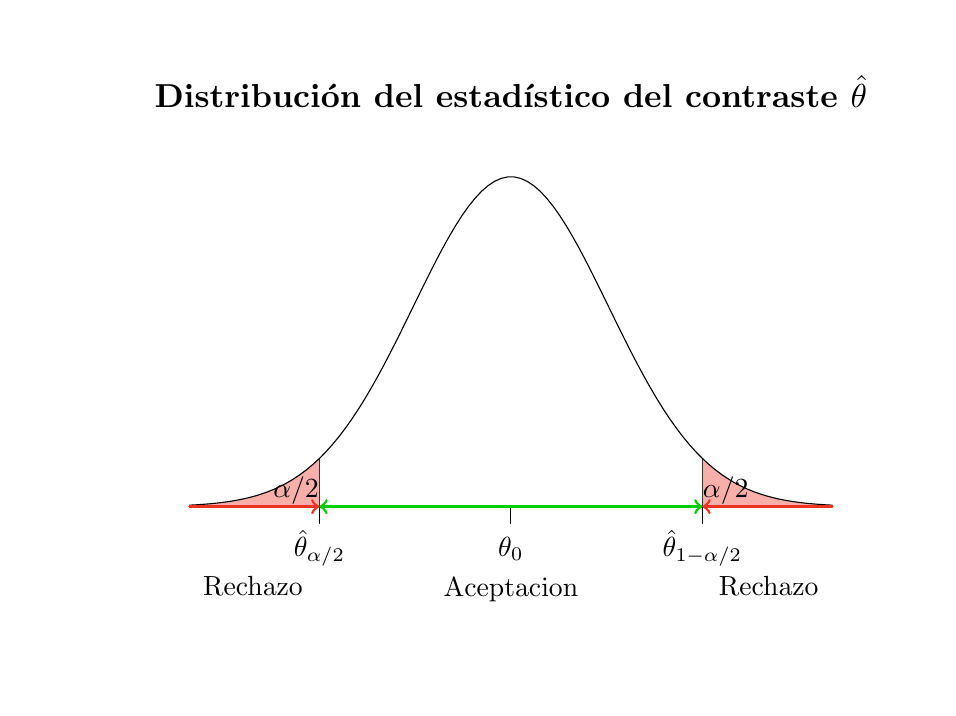
\begin{tikzpicture}[x=1pt,y=1pt]
\definecolor{fillColor}{RGB}{255,255,255}
\path[use as bounding box,fill=fillColor,fill opacity=0.00] (0,0) rectangle (325.21,238.49);
\begin{scope}
\path[clip] (  0.00,  0.00) rectangle (325.21,238.49);
\definecolor{drawColor}{RGB}{0,0,0}

\node[text=drawColor,anchor=base,inner sep=0pt, outer sep=0pt, scale=  1.20] at (174.61,209.75) {\bfseries Distribución del estadístico del contraste $\hat\theta$};
\end{scope}
\begin{scope}
\path[clip] (  0.00,  0.00) rectangle (325.21,238.49);
\definecolor{drawColor}{RGB}{0,0,0}

\path[draw=drawColor,line width= 0.4pt,line join=round,line cap=round] (105.41, 65.41) -- (243.81, 65.41);

\path[draw=drawColor,line width= 0.4pt,line join=round,line cap=round] (105.41, 65.41) -- (105.41, 59.41);

\path[draw=drawColor,line width= 0.4pt,line join=round,line cap=round] (174.61, 65.41) -- (174.61, 59.41);

\path[draw=drawColor,line width= 0.4pt,line join=round,line cap=round] (243.81, 65.41) -- (243.81, 59.41);

\node[text=drawColor,anchor=base,inner sep=0pt, outer sep=0pt, scale=  1.00] at (105.41, 47.41) {$\hat\theta_{\alpha/2}$};

\node[text=drawColor,anchor=base,inner sep=0pt, outer sep=0pt, scale=  1.00] at (174.61, 47.41) {$\theta_0$};

\node[text=drawColor,anchor=base,inner sep=0pt, outer sep=0pt, scale=  1.00] at (243.81, 47.41) {$\hat\theta_{1-\alpha/2}$};
\end{scope}
\begin{scope}
\path[clip] (  0.00,  0.00) rectangle (325.21,238.49);
\definecolor{fillColor}{RGB}{238,50,36}

\path[fill=fillColor,fill opacity=0.39] ( 58.49, 65.41) --
	( 58.49, 65.94) --
	( 60.84, 66.07) --
	( 63.18, 66.23) --
	( 65.53, 66.42) --
	( 67.87, 66.64) --
	( 70.22, 66.91) --
	( 72.56, 67.23) --
	( 74.91, 67.61) --
	( 77.26, 68.06) --
	( 79.60, 68.59) --
	( 81.95, 69.20) --
	( 84.29, 69.92) --
	( 86.64, 70.74) --
	( 88.99, 71.69) --
	( 91.33, 72.77) --
	( 93.68, 74.00) --
	( 96.02, 75.39) --
	( 98.37, 76.96) --
	(100.71, 78.71) --
	(103.06, 80.67) --
	(105.41, 82.83) --
	(105.41, 65.41) --
	cycle;

\path[fill=fillColor,fill opacity=0.39] (243.81, 65.41) --
	(243.81, 82.83) --
	(246.15, 80.67) --
	(248.50, 78.71) --
	(250.85, 76.96) --
	(253.19, 75.39) --
	(255.54, 74.00) --
	(257.88, 72.77) --
	(260.23, 71.69) --
	(262.58, 70.74) --
	(264.92, 69.92) --
	(267.27, 69.20) --
	(269.61, 68.59) --
	(271.96, 68.06) --
	(274.30, 67.61) --
	(276.65, 67.23) --
	(279.00, 66.91) --
	(281.34, 66.64) --
	(283.69, 66.42) --
	(286.03, 66.23) --
	(288.38, 66.07) --
	(290.73, 65.94) --
	(290.73, 65.41) --
	cycle;
\definecolor{drawColor}{gray}{0.20}

\path[draw=drawColor,line width= 0.4pt,line join=round,line cap=round] (105.41, 65.41) -- (105.41, 82.83);

\path[draw=drawColor,line width= 0.4pt,line join=round,line cap=round] (243.81, 65.41) -- (243.81, 82.83);
\definecolor{drawColor}{RGB}{0,0,0}

\path[draw=drawColor,line width= 0.4pt,line join=round,line cap=round] ( 58.49, 65.94) --
	( 60.84, 66.07) --
	( 63.18, 66.23) --
	( 65.53, 66.42) --
	( 67.87, 66.64) --
	( 70.22, 66.91) --
	( 72.56, 67.23) --
	( 74.91, 67.61) --
	( 77.26, 68.06) --
	( 79.60, 68.59) --
	( 81.95, 69.20) --
	( 84.29, 69.92) --
	( 86.64, 70.74) --
	( 88.99, 71.69) --
	( 91.33, 72.77) --
	( 93.68, 74.00) --
	( 96.02, 75.39) --
	( 98.37, 76.96) --
	(100.71, 78.71) --
	(103.06, 80.67) --
	(105.41, 82.83) --
	(107.75, 85.21) --
	(110.10, 87.82) --
	(112.44, 90.66) --
	(114.79, 93.74) --
	(117.13, 97.05) --
	(119.48,100.59) --
	(121.83,104.35) --
	(124.17,108.33) --
	(126.52,112.50) --
	(128.86,116.85) --
	(131.21,121.36) --
	(133.56,125.99) --
	(135.90,130.72) --
	(138.25,135.51) --
	(140.59,140.31) --
	(142.94,145.09) --
	(145.28,149.81) --
	(147.63,154.40) --
	(149.98,158.84) --
	(152.32,163.06) --
	(154.67,167.02) --
	(157.01,170.68) --
	(159.36,173.99) --
	(161.71,176.90) --
	(164.05,179.40) --
	(166.40,181.43) --
	(168.74,182.98) --
	(171.09,184.02) --
	(173.43,184.55) --
	(175.78,184.55) --
	(178.13,184.02) --
	(180.47,182.98) --
	(182.82,181.43) --
	(185.16,179.40) --
	(187.51,176.90) --
	(189.86,173.99) --
	(192.20,170.68) --
	(194.55,167.02) --
	(196.89,163.06) --
	(199.24,158.84) --
	(201.58,154.40) --
	(203.93,149.81) --
	(206.28,145.09) --
	(208.62,140.31) --
	(210.97,135.51) --
	(213.31,130.72) --
	(215.66,125.99) --
	(218.01,121.36) --
	(220.35,116.85) --
	(222.70,112.50) --
	(225.04,108.33) --
	(227.39,104.35) --
	(229.73,100.59) --
	(232.08, 97.05) --
	(234.43, 93.74) --
	(236.77, 90.66) --
	(239.12, 87.82) --
	(241.46, 85.21) --
	(243.81, 82.83) --
	(246.15, 80.67) --
	(248.50, 78.71) --
	(250.85, 76.96) --
	(253.19, 75.39) --
	(255.54, 74.00) --
	(257.88, 72.77) --
	(260.23, 71.69) --
	(262.58, 70.74) --
	(264.92, 69.92) --
	(267.27, 69.20) --
	(269.61, 68.59) --
	(271.96, 68.06) --
	(274.30, 67.61) --
	(276.65, 67.23) --
	(279.00, 66.91) --
	(281.34, 66.64) --
	(283.69, 66.42) --
	(286.03, 66.23) --
	(288.38, 66.07) --
	(290.73, 65.94);

\node[text=drawColor,anchor=base,inner sep=0pt, outer sep=0pt, scale=  1.00] at ( 96.98, 68.89) {$\alpha/2$};

\node[text=drawColor,anchor=base,inner sep=0pt, outer sep=0pt, scale=  1.00] at (252.23, 68.89) {$\alpha/2$};

\node[text=drawColor,anchor=base,inner sep=0pt, outer sep=0pt, scale=  1.00] at (174.61, 33.06) {Aceptacion};

\node[text=drawColor,anchor=base east,inner sep=0pt, outer sep=0pt, scale=  1.00] at ( 99.41, 33.24) {Rechazo};

\node[text=drawColor,anchor=base west,inner sep=0pt, outer sep=0pt, scale=  1.00] at (249.81, 33.24) {Rechazo};
\definecolor{drawColor}{RGB}{238,50,36}

\path[->, draw=drawColor,line width= 1pt,line join=round,line cap=round] ( 58.49, 65.41) -- (105.41, 65.41);
\definecolor{drawColor}{RGB}{0,205,0}

\path[<->, draw=drawColor,line width= 1pt,line join=round,line cap=round] (105.41, 65.41) -- (243.81, 65.41);
\definecolor{drawColor}{RGB}{238,50,36}

\path[->, draw=drawColor,line width= 1pt,line join=round,line cap=round] (290.73, 65.41) -- (243.81, 65.41);
\end{scope}
\end{tikzpicture}
